\documentclass[]{article}
\usepackage{lmodern}
\usepackage{amssymb,amsmath}
\usepackage{ifxetex,ifluatex}
\usepackage{fixltx2e} % provides \textsubscript
\ifnum 0\ifxetex 1\fi\ifluatex 1\fi=0 % if pdftex
  \usepackage[T1]{fontenc}
  \usepackage[utf8]{inputenc}
\else % if luatex or xelatex
  \ifxetex
    \usepackage{mathspec}
    \usepackage{xltxtra,xunicode}
  \else
    \usepackage{fontspec}
  \fi
  \defaultfontfeatures{Mapping=tex-text,Scale=MatchLowercase}
  \newcommand{\euro}{€}
\fi
% use upquote if available, for straight quotes in verbatim environments
\IfFileExists{upquote.sty}{\usepackage{upquote}}{}
% use microtype if available
\IfFileExists{microtype.sty}{%
\usepackage{microtype}
\UseMicrotypeSet[protrusion]{basicmath} % disable protrusion for tt fonts
}{}
\usepackage[margin=1in]{geometry}
\usepackage{color}
\usepackage{fancyvrb}
\newcommand{\VerbBar}{|}
\newcommand{\VERB}{\Verb[commandchars=\\\{\}]}
\DefineVerbatimEnvironment{Highlighting}{Verbatim}{commandchars=\\\{\}}
% Add ',fontsize=\small' for more characters per line
\usepackage{framed}
\definecolor{shadecolor}{RGB}{248,248,248}
\newenvironment{Shaded}{\begin{snugshade}}{\end{snugshade}}
\newcommand{\KeywordTok}[1]{\textcolor[rgb]{0.13,0.29,0.53}{\textbf{{#1}}}}
\newcommand{\DataTypeTok}[1]{\textcolor[rgb]{0.13,0.29,0.53}{{#1}}}
\newcommand{\DecValTok}[1]{\textcolor[rgb]{0.00,0.00,0.81}{{#1}}}
\newcommand{\BaseNTok}[1]{\textcolor[rgb]{0.00,0.00,0.81}{{#1}}}
\newcommand{\FloatTok}[1]{\textcolor[rgb]{0.00,0.00,0.81}{{#1}}}
\newcommand{\CharTok}[1]{\textcolor[rgb]{0.31,0.60,0.02}{{#1}}}
\newcommand{\StringTok}[1]{\textcolor[rgb]{0.31,0.60,0.02}{{#1}}}
\newcommand{\CommentTok}[1]{\textcolor[rgb]{0.56,0.35,0.01}{\textit{{#1}}}}
\newcommand{\OtherTok}[1]{\textcolor[rgb]{0.56,0.35,0.01}{{#1}}}
\newcommand{\AlertTok}[1]{\textcolor[rgb]{0.94,0.16,0.16}{{#1}}}
\newcommand{\FunctionTok}[1]{\textcolor[rgb]{0.00,0.00,0.00}{{#1}}}
\newcommand{\RegionMarkerTok}[1]{{#1}}
\newcommand{\ErrorTok}[1]{\textbf{{#1}}}
\newcommand{\NormalTok}[1]{{#1}}
\usepackage{graphicx}
\makeatletter
\def\maxwidth{\ifdim\Gin@nat@width>\linewidth\linewidth\else\Gin@nat@width\fi}
\def\maxheight{\ifdim\Gin@nat@height>\textheight\textheight\else\Gin@nat@height\fi}
\makeatother
% Scale images if necessary, so that they will not overflow the page
% margins by default, and it is still possible to overwrite the defaults
% using explicit options in \includegraphics[width, height, ...]{}
\setkeys{Gin}{width=\maxwidth,height=\maxheight,keepaspectratio}
\ifxetex
  \usepackage[setpagesize=false, % page size defined by xetex
              unicode=false, % unicode breaks when used with xetex
              xetex]{hyperref}
\else
  \usepackage[unicode=true]{hyperref}
\fi
\hypersetup{breaklinks=true,
            bookmarks=true,
            pdfauthor={JcB},
            pdftitle={Analyse le fichier mergé},
            colorlinks=true,
            citecolor=blue,
            urlcolor=blue,
            linkcolor=magenta,
            pdfborder={0 0 0}}
\urlstyle{same}  % don't use monospace font for urls
\setlength{\parindent}{0pt}
\setlength{\parskip}{6pt plus 2pt minus 1pt}
\setlength{\emergencystretch}{3em}  % prevent overfull lines
\setcounter{secnumdepth}{5}

%%% Use protect on footnotes to avoid problems with footnotes in titles
\let\rmarkdownfootnote\footnote%
\def\footnote{\protect\rmarkdownfootnote}

%%% Change title format to be more compact
\usepackage{titling}

% Create subtitle command for use in maketitle
\newcommand{\subtitle}[1]{
  \posttitle{
    \begin{center}\large#1\end{center}
    }
}

\setlength{\droptitle}{-2em}
  \title{Analyse le fichier mergé}
  \pretitle{\vspace{\droptitle}\centering\huge}
  \posttitle{\par}
  \author{JcB}
  \preauthor{\centering\large\emph}
  \postauthor{\par}
  \predate{\centering\large\emph}
  \postdate{\par}
  \date{22/11/2015}



\begin{document}

\maketitle


{
\hypersetup{linkcolor=black}
\setcounter{tocdepth}{2}
\tableofcontents
}
Alalyse le fichier \textbf{merge2015} résultant du merging des fichiers
\textbf{dpr2} et \textbf{orumip}. Voir README.md pour la signification
des fichiers. Le fichier \emph{merge2015} est par
\textbf{Analyse\_regroupement}.

\section{Récupération des fichiers de
travail}\label{recuperation-des-fichiers-de-travail}

\begin{Shaded}
\begin{Highlighting}[]
\KeywordTok{library}\NormalTok{(epicalc)}
\end{Highlighting}
\end{Shaded}

\begin{verbatim}
## Loading required package: foreign
\end{verbatim}

\begin{verbatim}
## Loading required package: survival
\end{verbatim}

\begin{verbatim}
## Loading required package: MASS
\end{verbatim}

\begin{verbatim}
## Loading required package: nnet
\end{verbatim}

\begin{Shaded}
\begin{Highlighting}[]
\NormalTok{path <-}\StringTok{ "../"} \CommentTok{# path <- "" en mode console}

\KeywordTok{load}\NormalTok{(}\StringTok{"../Analyse_regroupements/merge2015.Rda"}\NormalTok{) }\CommentTok{# le fichier mergé}
\KeywordTok{source}\NormalTok{(}\KeywordTok{paste0}\NormalTok{(path,}\StringTok{"regroupement.R"}\NormalTok{))}

\NormalTok{d3 <-}\StringTok{ }\NormalTok{merge2015 }\CommentTok{# pour rendre le programme générique}
\NormalTok{anc <-}\StringTok{ }\DecValTok{2015}

\KeywordTok{names}\NormalTok{(d3)}
\end{Highlighting}
\end{Shaded}

\begin{verbatim}
##  [1] "DP"            "id"            "CODE_POSTAL"   "COMMUNE"      
##  [5] "DESTINATION"   "ENTREE"        "EXTRACT"       "FINESS"       
##  [9] "GRAVITE"       "MODE_ENTREE"   "MODE_SORTIE"   "MOTIF"        
## [13] "NAISSANCE"     "ORIENTATION"   "PROVENANCE"    "SEXE"         
## [17] "SORTIE"        "TRANSPORT"     "TRANSPORT_PEC" "AGE"          
## [21] "LIBELLE_CIM10" "SFMU"          "TYPE_URGENCES" "CHAPITRE"     
## [25] "SOUS_CHAPITRE"
\end{verbatim}

\begin{Shaded}
\begin{Highlighting}[]
\KeywordTok{summary}\NormalTok{(d3$TYPE_URGENCES)}
\end{Highlighting}
\end{Shaded}

\begin{verbatim}
##      Autre recours Médico-chirurgical      Psychiatrique 
##               9500             177017               6803 
##      Toxicologique    Traumatologique               NA's 
##               4900             116334                359
\end{verbatim}

\begin{Shaded}
\begin{Highlighting}[]
\CommentTok{# Décommenter si nécessaire. Affichage volumineux}
\CommentTok{# summary(d3$CHAPITRE)}
\CommentTok{# summary(d3$SOUS_CHAPITRE)}

\KeywordTok{tapply}\NormalTok{(d3$TYPE_URGENCES, }\KeywordTok{list}\NormalTok{(d3$FINESS, d3$TYPE_URGENCES), length)}
\end{Highlighting}
\end{Shaded}

\begin{verbatim}
##     Autre recours Médico-chirurgical Psychiatrique Toxicologique
## 3Fr           608               5703           192            83
## Alk           188               1322            59            18
## Ane            NA                 NA            NA            NA
## Col          2564              30275          1627          1063
## Dia           632               7497           125             7
## Dts            NA               1736            NA            NA
## Geb           619               7117           142           124
## Hag           851              21316           551           545
## Hus            NA                 NA            NA            NA
## Mul          1056              18671          1416           696
## Odi           116               8299            57             2
## Ros            NA                 NA            NA            NA
## Sav           173               3468           165            90
## Sel           909              13609           296           409
## Wis           475               6350           241           110
## HTP           524              27497           612           597
## NHC           170              12061           327           658
## Emr           509               7715           943           452
## Hsr           106               4381            50            46
## Ccm            NA                 NA            NA            NA
##     Traumatologique
## 3Fr            4220
## Alk            1506
## Ane              NA
## Col           22380
## Dia            4911
## Dts            6448
## Geb            7763
## Hag           12623
## Hus              NA
## Mul            7819
## Odi            3725
## Ros             574
## Sav            3495
## Sel           12828
## Wis            4488
## HTP           17495
## NHC             757
## Emr            5284
## Hsr              18
## Ccm              NA
\end{verbatim}

\subsection{Type d'urgence}\label{type-durgence}

\begin{Shaded}
\begin{Highlighting}[]
\NormalTok{n.type <-}\StringTok{ }\KeywordTok{nrow}\NormalTok{(d3)}
\NormalTok{s.type <-}\StringTok{ }\KeywordTok{summary}\NormalTok{(d3$TYPE_URGENCES)}
\NormalTok{s.type}
\end{Highlighting}
\end{Shaded}

\begin{verbatim}
##      Autre recours Médico-chirurgical      Psychiatrique 
##               9500             177017               6803 
##      Toxicologique    Traumatologique               NA's 
##               4900             116334                359
\end{verbatim}

\begin{Shaded}
\begin{Highlighting}[]
\KeywordTok{pie}\NormalTok{(s.type, }\DataTypeTok{main =} \KeywordTok{paste0}\NormalTok{(anc, }\StringTok{" - Grands groupes diagnostics"}\NormalTok{), }\DataTypeTok{col =} \KeywordTok{c}\NormalTok{(}\StringTok{"yellow"}\NormalTok{,}\StringTok{"blue"}\NormalTok{, }\StringTok{"orange"}\NormalTok{, }\StringTok{"green"}\NormalTok{, }\StringTok{"red"}\NormalTok{,}\StringTok{"black"}\NormalTok{))}
\end{Highlighting}
\end{Shaded}

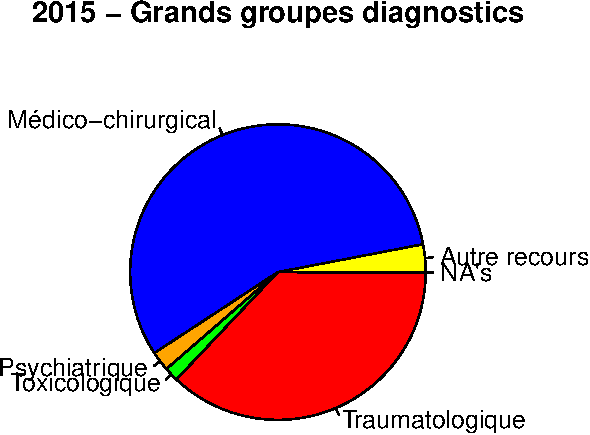
\includegraphics{analyse_merge_files/figure-latex/type_urgence-1.pdf}\\

\begin{Shaded}
\begin{Highlighting}[]
\KeywordTok{par}\NormalTok{(}\DataTypeTok{mar =} \KeywordTok{c}\NormalTok{(}\DecValTok{6}\NormalTok{,}\DecValTok{4}\NormalTok{,}\DecValTok{3}\NormalTok{,}\DecValTok{2}\NormalTok{))}
\KeywordTok{barplot}\NormalTok{(}\KeywordTok{sort}\NormalTok{(s.type, }\DataTypeTok{decreasing =} \OtherTok{TRUE}\NormalTok{), }\DataTypeTok{las =} \DecValTok{2}\NormalTok{, }\DataTypeTok{cex.names =} \FloatTok{0.7}\NormalTok{, }\DataTypeTok{main =} \StringTok{"Répartition des diagnostics principaux }\CharTok{\textbackslash{}n}\StringTok{selon les codes de regroupement de l' ORUMIP"}\NormalTok{)}
\end{Highlighting}
\end{Shaded}

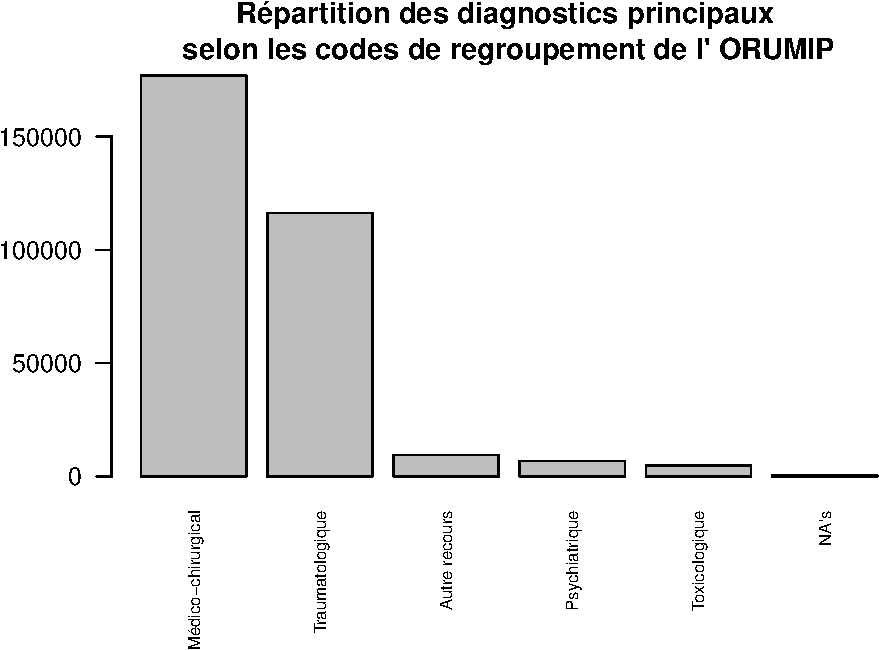
\includegraphics{analyse_merge_files/figure-latex/type_urgence-2.pdf}\\

\begin{Shaded}
\begin{Highlighting}[]
\KeywordTok{tab1}\NormalTok{(d3$TYPE_URGENCES, }\DataTypeTok{sort.group =} \StringTok{"decreasing"}\NormalTok{, }\DataTypeTok{cex.names =} \FloatTok{0.6}\NormalTok{, }\DataTypeTok{main =} \StringTok{"Répartition des diagnostics principaux }\CharTok{\textbackslash{}n}\StringTok{selon les codes de regroupement de l' ORUMIP"}\NormalTok{)}
\end{Highlighting}
\end{Shaded}

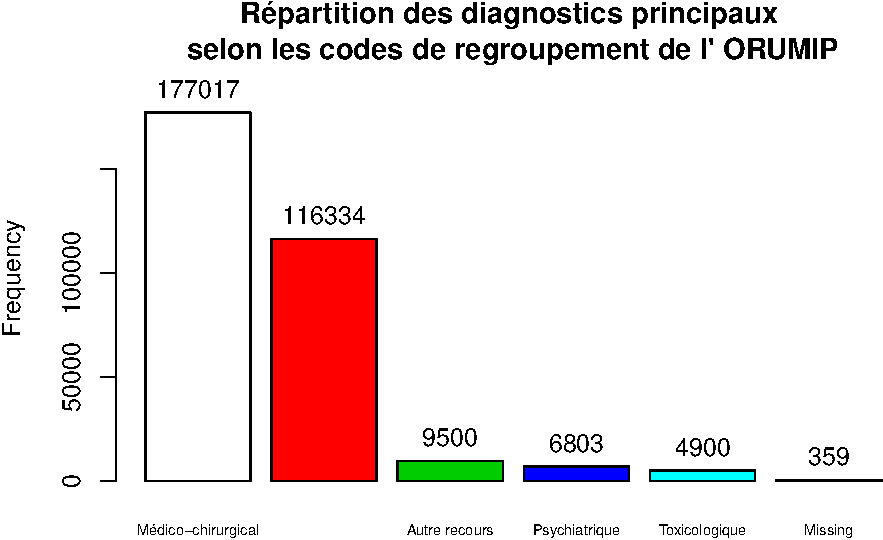
\includegraphics{analyse_merge_files/figure-latex/type_urgence-3.pdf}\\

\begin{verbatim}
## d3$TYPE_URGENCES : 
##                    Frequency   %(NA+)   %(NA-)
## Médico-chirurgical    177017     56.2     56.3
## Traumatologique       116334     36.9     37.0
## Autre recours           9500      3.0      3.0
## Psychiatrique           6803      2.2      2.2
## Toxicologique           4900      1.6      1.6
## NA's                     359      0.1      0.0
##   Total               314913    100.0    100.0
\end{verbatim}

359 codes de sont pas reconnus (0.11 \%).

\begin{Shaded}
\begin{Highlighting}[]
\NormalTok{a <-}\StringTok{ }\NormalTok{d3[}\KeywordTok{is.na}\NormalTok{(d3$TYPE_URGENCES),]}
\KeywordTok{cbind}\NormalTok{(}\KeywordTok{summary}\NormalTok{(}\KeywordTok{as.factor}\NormalTok{(a$DP)))}
\end{Highlighting}
\end{Shaded}

\begin{verbatim}
##                     [,1]
## I200+                 12
## N23 0                 11
## W5700                  9
## W0689                  6
## X6591                  6
## V4259                  5
## W1008                  5
## W5701                  5
## W0709                  4
## W1929                  4
## W5799                  4
## Y1509                  4
## M459                   3
## T16 0                  3
## V1938                  3
## V4269                  3
## W1959                  3
## W5709                  3
## W5781                  3
## Y3341                  3
## Y3343                  3
## Z                      3
## S011 02                2
## S2250+B6               2
## V1328                  2
## V1941                  2
## V4859                  2
## W0184                  2
## W0608                  2
## W0694                  2
## W0704                  2
## W1048                  2
## W1998                  2
## W4483                  2
## W4581                  2
## W5434                  2
## W5703                  2
## W5704                  2
## W5743                  2
## X2302                  2
## X4420                  2
## X4548                  2
## X4594                  2
## X6102                  2
## X6434                  2
## X6549                  2
## X6592                  2
## Y0422                  2
## Y0449                  2
## Y1559                  2
## Z0488                  2
## Z6030                  2
## F034                   1
## G510 02                1
## GH819) VERTIGES        1
## J90 0                  1
## JJ189) PNEUMOPATHIE    1
## K409 01                1
## MM199) ARTHROSE SP     1
## MM255) ARTHRALGIES     1
## NN419) PROSTATITE      1
## PW199) CHUTE           1
## S202 02                1
## S223 01                1
## S372(0                 1
## S422 02                1
## S720 02                1
## S729 01                1
## S800 01                1
## S801 02                1
## S823 01                1
## S929 01                1
## SS331                  1
## SV899) AVP             1
## SY099) AGRESSION       1
## U152                   1
## V0100                  1
## V0408                  1
## V1149                  1
## V1293                  1
## V1358                  1
## V1931                  1
## V2658                  1
## V4008                  1
## V4053                  1
## V4202                  1
## V4211                  1
## V4654                  1
## V5201                  1
## V5351                  1
## V7894                  1
## V9312                  1
## W0104                  1
## W0123                  1
## W0218                  1
## W0458                  1
## W0604                  1
## W0609                  1
## W0620                  1
## (Other)              147
\end{verbatim}

\begin{itemize}
\itemsep1pt\parskip0pt\parsep0pt
\item
  Plus de la moitié des codes concernent \textbf{R53+0}, \textbf{R53+1}
  et \textbf{R53+2} qui sont des codes PMSI. \emph{R53} = Malaise et
  fatigue.
\item
  r11 = vomissements: pb de casse
\item
  B99+1 = Syndrome infectieux sans cause trouvée
\end{itemize}

exemple pour Mulhouse:

\begin{Shaded}
\begin{Highlighting}[]
\NormalTok{mul <-}\StringTok{ }\NormalTok{merge2015[}\KeywordTok{is.na}\NormalTok{(merge2015$LIBELLE_CIM10) &}\StringTok{ }\NormalTok{merge2015$FINESS %in%}\StringTok{ }\KeywordTok{c}\NormalTok{(}\StringTok{"Mul"}\NormalTok{,}\StringTok{"Hsr"}\NormalTok{,}\StringTok{"Emr"}\NormalTok{),]}
\NormalTok{mulx <-}\StringTok{ }\KeywordTok{cbind}\NormalTok{(}\KeywordTok{summary}\NormalTok{(}\KeywordTok{as.factor}\NormalTok{(mul$DP)))}
\NormalTok{mulx}
\end{Highlighting}
\end{Shaded}

\begin{verbatim}
##                     [,1]
## GH819) VERTIGES        1
## JJ189) PNEUMOPATHIE    1
## M459                   3
## MM199) ARTHROSE SP     1
## MM255) ARTHRALGIES     1
## NN419) PROSTATITE      1
## PW199) CHUTE           1
## S2250+B6               2
## S372(0                 1
## SV899) AVP             1
## SY099) AGRESSION       1
## Z                      3
\end{verbatim}

\section{Par type d'urgence}\label{par-type-durgence}

Le regroupement principal de l'ORUMIP comprend les chapitres suivants:

\begin{verbatim}
[1] "Autre recours"      "Médico-chirurgical" "Psychiatrique"     
[4] "Toxicologique"      "Traumatologique"   
\end{verbatim}

\subsection{Analyse des urgences
médico-chirurgicales}\label{analyse-des-urgences-medico-chirurgicales}

\begin{Shaded}
\begin{Highlighting}[]
\NormalTok{s.type <-}\StringTok{ }\KeywordTok{summary}\NormalTok{(d3$TYPE_URGENCES)}
\KeywordTok{sort}\NormalTok{(s.type, }\DataTypeTok{decreasing =} \OtherTok{TRUE}\NormalTok{)}
\end{Highlighting}
\end{Shaded}

\begin{verbatim}
## Médico-chirurgical    Traumatologique      Autre recours 
##             177017             116334               9500 
##      Psychiatrique      Toxicologique               NA's 
##               6803               4900                359
\end{verbatim}

\begin{Shaded}
\begin{Highlighting}[]
\NormalTok{medic <-}\StringTok{ }\NormalTok{d3[d3$TYPE_URGENCES ==}\StringTok{ "Médico-chirurgical"}\NormalTok{,]}

\KeywordTok{tab1}\NormalTok{(}\KeywordTok{factor}\NormalTok{(medic$CHAPITRE), }\DataTypeTok{sort.group =} \StringTok{"decreasing"}\NormalTok{, }\DataTypeTok{bar.values =} \StringTok{"percent"}\NormalTok{, }\DataTypeTok{cex.names =} \FloatTok{0.8}\NormalTok{, }\DataTypeTok{main =} \StringTok{"Médico-chirurgical"}\NormalTok{)}
\end{Highlighting}
\end{Shaded}

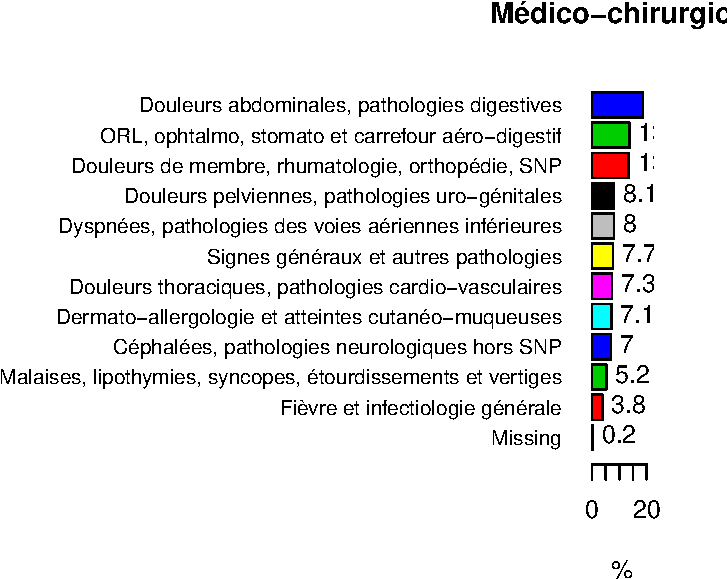
\includegraphics{analyse_merge_files/figure-latex/chapitre-1.pdf}\\

\begin{verbatim}
## factor(medic$CHAPITRE) : 
##                                                              Frequency
## Douleurs abdominales, pathologies digestives                     32849
## ORL, ophtalmo, stomato et carrefour aéro-digestif                24846
## Douleurs de membre, rhumatologie, orthopédie, SNP                23911
## Dyspnées, pathologies des voies aériennes inférieures            14621
## Douleurs pelviennes, pathologies uro-génitales                   14239
## Signes généraux et autres pathologies                            13314
## Douleurs thoraciques, pathologies cardio-vasculaires             13179
## Dermato-allergologie et atteintes cutanéo-muqueuses              12286
## Céphalées, pathologies neurologiques hors SNP                    12256
## Malaises, lipothymies, syncopes, étourdissements et vertiges      9027
## Fièvre et infectiologie générale                                  6489
## NA's                                                               359
##   Total                                                         177376
##                                                                %(NA+)
## Douleurs abdominales, pathologies digestives                     18.5
## ORL, ophtalmo, stomato et carrefour aéro-digestif                14.0
## Douleurs de membre, rhumatologie, orthopédie, SNP                13.5
## Dyspnées, pathologies des voies aériennes inférieures             8.2
## Douleurs pelviennes, pathologies uro-génitales                    8.0
## Signes généraux et autres pathologies                             7.5
## Douleurs thoraciques, pathologies cardio-vasculaires              7.4
## Dermato-allergologie et atteintes cutanéo-muqueuses               6.9
## Céphalées, pathologies neurologiques hors SNP                     6.9
## Malaises, lipothymies, syncopes, étourdissements et vertiges      5.1
## Fièvre et infectiologie générale                                  3.7
## NA's                                                              0.2
##   Total                                                         100.0
##                                                                %(NA-)
## Douleurs abdominales, pathologies digestives                     18.6
## ORL, ophtalmo, stomato et carrefour aéro-digestif                14.0
## Douleurs de membre, rhumatologie, orthopédie, SNP                13.5
## Dyspnées, pathologies des voies aériennes inférieures             8.3
## Douleurs pelviennes, pathologies uro-génitales                    8.0
## Signes généraux et autres pathologies                             7.5
## Douleurs thoraciques, pathologies cardio-vasculaires              7.4
## Dermato-allergologie et atteintes cutanéo-muqueuses               6.9
## Céphalées, pathologies neurologiques hors SNP                     6.9
## Malaises, lipothymies, syncopes, étourdissements et vertiges      5.1
## Fièvre et infectiologie générale                                  3.7
## NA's                                                              0.0
##   Total                                                         100.0
\end{verbatim}

\subsection{Analyse des urgences
médico-chirurgicales}\label{analyse-des-urgences-medico-chirurgicales-1}

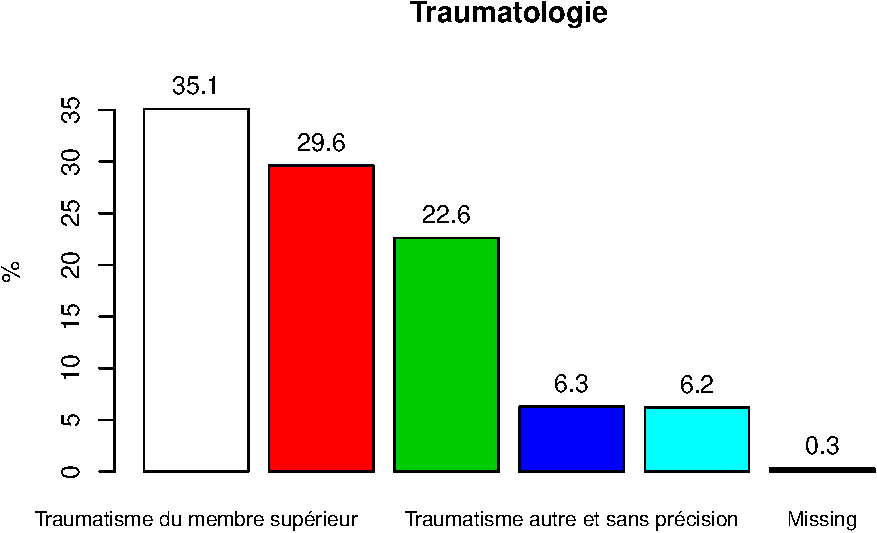
\includegraphics{analyse_merge_files/figure-latex/urg_traumato-1.pdf}\\

\begin{verbatim}
## factor(trauma$CHAPITRE) : 
##                                      Frequency   %(NA+)   %(NA-)
## Traumatisme du membre supérieur          40914     35.1     35.2
## Traumatisme du membre inférieur          34529     29.6     29.7
## Traumatisme de la tête et du cou         26407     22.6     22.7
## Traumatisme autre et sans précision       7295      6.3      6.3
## Traumatisme thoraco-abdomino-pelvien      7189      6.2      6.2
## NA's                                       359      0.3      0.0
##   Total                                 116693    100.0    100.0
\end{verbatim}

\section{Par age}\label{par-age}

\subsection{Adultes (18 à 75 ans)}\label{adultes-18-a-75-ans}

\begin{Shaded}
\begin{Highlighting}[]
\NormalTok{d3a <-}\StringTok{ }\NormalTok{d3[d3$AGE >}\StringTok{ }\DecValTok{17} \NormalTok{&}\StringTok{ }\NormalTok{d3$AGE <}\StringTok{ }\DecValTok{76}\NormalTok{,]}
\NormalTok{n.adl <-}\StringTok{ }\KeywordTok{nrow}\NormalTok{(d3a)}

\CommentTok{# table fréquence}
\NormalTok{s.type.adl <-}\StringTok{ }\KeywordTok{table}\NormalTok{(d3a$TYPE_URGENCES)}
\NormalTok{s.type.adl}
\end{Highlighting}
\end{Shaded}

\begin{verbatim}
## 
##      Autre recours Médico-chirurgical      Psychiatrique 
##               6298              95992               5423 
##      Toxicologique    Traumatologique 
##               4167              62025
\end{verbatim}

\begin{Shaded}
\begin{Highlighting}[]
\CommentTok{# table des proportion}
\NormalTok{p.type.adl <-}\StringTok{ }\KeywordTok{round}\NormalTok{(}\KeywordTok{prop.table}\NormalTok{(s.type.adl) *}\StringTok{ }\DecValTok{100}\NormalTok{, }\DecValTok{2}\NormalTok{)}
\NormalTok{p.type.adl}
\end{Highlighting}
\end{Shaded}

\begin{verbatim}
## 
##      Autre recours Médico-chirurgical      Psychiatrique 
##               3.62              55.20               3.12 
##      Toxicologique    Traumatologique 
##               2.40              35.67
\end{verbatim}

\begin{Shaded}
\begin{Highlighting}[]
\KeywordTok{pie}\NormalTok{(s.type.adl, }\DataTypeTok{main =} \StringTok{"Adultes"}\NormalTok{, }\DataTypeTok{cex=}\FloatTok{0.8}\NormalTok{, }\DataTypeTok{col =} \KeywordTok{palette}\NormalTok{(}\KeywordTok{heat.colors}\NormalTok{(}\DecValTok{6}\NormalTok{)))}
\end{Highlighting}
\end{Shaded}

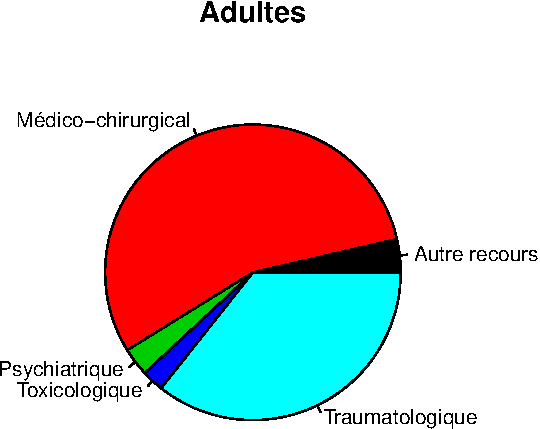
\includegraphics{analyse_merge_files/figure-latex/adultes-1.pdf}\\

\begin{Shaded}
\begin{Highlighting}[]
\NormalTok{taba <-}\StringTok{ }\KeywordTok{tab1}\NormalTok{(d3a$TYPE_URGENCES, }\DataTypeTok{sort.group =} \StringTok{"decreasing"}\NormalTok{, }\DataTypeTok{bar.values =} \StringTok{"percent"}\NormalTok{, }\DataTypeTok{cex.names =} \FloatTok{0.8}\NormalTok{, }\DataTypeTok{main =} \KeywordTok{paste0}\NormalTok{(}\StringTok{"Médico-chirurgical adulte (N = "}\NormalTok{, n.adl, }\StringTok{")"}\NormalTok{), }\DataTypeTok{missing =} \OtherTok{FALSE}\NormalTok{)}
\end{Highlighting}
\end{Shaded}

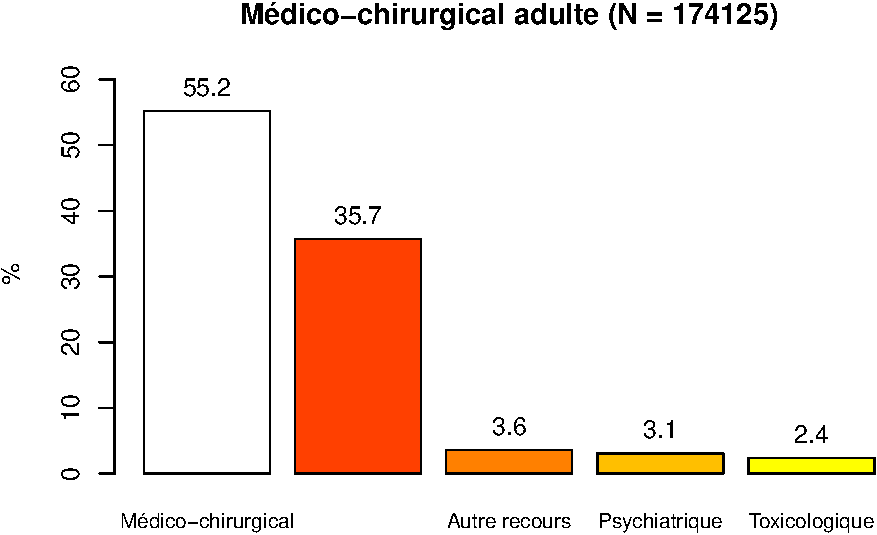
\includegraphics{analyse_merge_files/figure-latex/adultes-2.pdf}\\

\subsection{Pédiatrie (age \textless{} 18
ans)}\label{pediatrie-age-18-ans}

\begin{Shaded}
\begin{Highlighting}[]
\NormalTok{d3p <-}\StringTok{ }\NormalTok{d3[d3$AGE <}\StringTok{ }\DecValTok{18}\NormalTok{,]}
\NormalTok{n.ped<-}\StringTok{ }\KeywordTok{nrow}\NormalTok{(d3p)}

\NormalTok{s.type.ped <-}\StringTok{ }\KeywordTok{table}\NormalTok{(d3p$TYPE_URGENCES)}
\KeywordTok{sort}\NormalTok{(s.type.ped, }\DataTypeTok{decreasing =} \OtherTok{TRUE}\NormalTok{)}
\end{Highlighting}
\end{Shaded}

\begin{verbatim}
## 
## Médico-chirurgical    Traumatologique      Autre recours 
##              54620              44213               2559 
##      Psychiatrique      Toxicologique 
##                924                547
\end{verbatim}

\begin{Shaded}
\begin{Highlighting}[]
\KeywordTok{pie}\NormalTok{(s.type.ped, }\DataTypeTok{main =} \StringTok{"Pédiatrie"}\NormalTok{, }\DataTypeTok{cex=}\FloatTok{0.8}\NormalTok{, }\DataTypeTok{col =} \KeywordTok{palette}\NormalTok{(}\KeywordTok{heat.colors}\NormalTok{(}\DecValTok{6}\NormalTok{)))}
\end{Highlighting}
\end{Shaded}

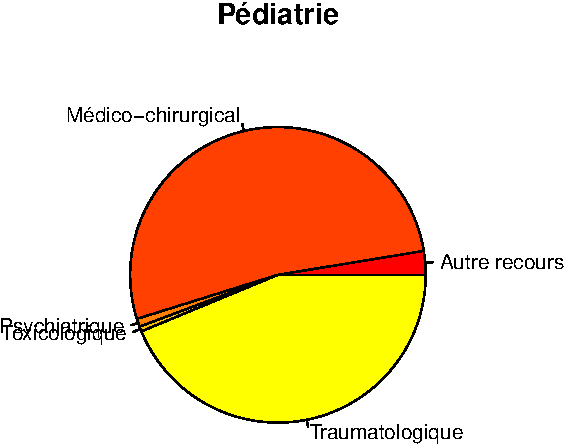
\includegraphics{analyse_merge_files/figure-latex/ped-1.pdf}\\

\begin{Shaded}
\begin{Highlighting}[]
\NormalTok{tabp <-}\StringTok{ }\KeywordTok{tab1}\NormalTok{(d3p$TYPE_URGENCES, }\DataTypeTok{sort.group =} \StringTok{"decreasing"}\NormalTok{, }\DataTypeTok{bar.values =} \StringTok{"percent"}\NormalTok{, }\DataTypeTok{cex.names =} \FloatTok{0.8}\NormalTok{, }\DataTypeTok{main =} \KeywordTok{paste0}\NormalTok{(}\StringTok{"Médico-chirurgical pédiatrique (N = "}\NormalTok{, n.ped, }\StringTok{")"}\NormalTok{), }\DataTypeTok{missing =} \OtherTok{FALSE}\NormalTok{)}
\end{Highlighting}
\end{Shaded}

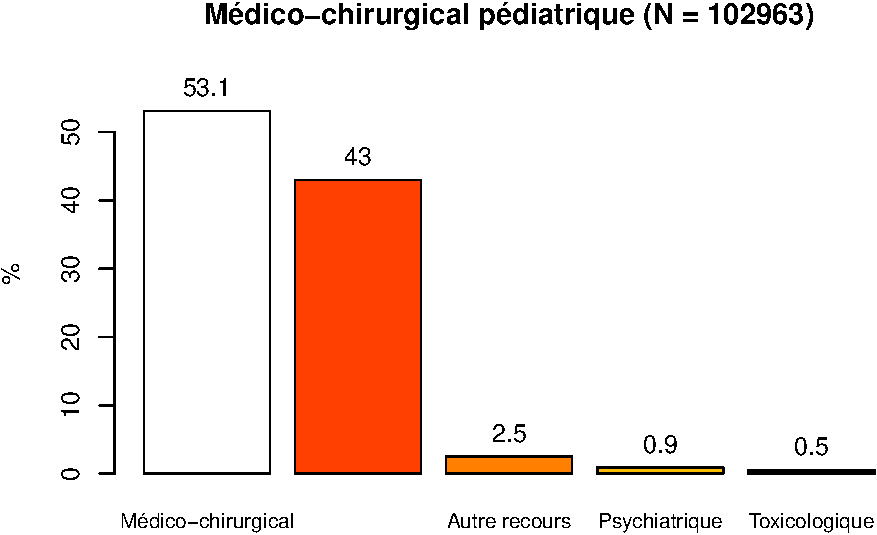
\includegraphics{analyse_merge_files/figure-latex/ped-2.pdf}\\ Gériatrie
(age \textgreater{} 75 ans) ------------------------

\begin{Shaded}
\begin{Highlighting}[]
\NormalTok{d3g <-}\StringTok{ }\NormalTok{d3[d3$AGE >}\StringTok{ }\DecValTok{75}\NormalTok{,]}
\NormalTok{n.ger <-}\StringTok{ }\KeywordTok{nrow}\NormalTok{(d3g)}

\NormalTok{s.type.ger <-}\StringTok{ }\KeywordTok{table}\NormalTok{(d3g$TYPE_URGENCES)}
\KeywordTok{sort}\NormalTok{(s.type.ger, }\DataTypeTok{decreasing =} \OtherTok{TRUE}\NormalTok{)}
\end{Highlighting}
\end{Shaded}

\begin{verbatim}
## 
## Médico-chirurgical    Traumatologique      Autre recours 
##              26405              10096                643 
##      Psychiatrique      Toxicologique 
##                454                186
\end{verbatim}

\begin{Shaded}
\begin{Highlighting}[]
\KeywordTok{pie}\NormalTok{(}\KeywordTok{sort}\NormalTok{(s.type.ger), }\DataTypeTok{main =} \StringTok{"Gériatrie"}\NormalTok{, }\DataTypeTok{cex=}\FloatTok{0.8}\NormalTok{, }\DataTypeTok{col =} \KeywordTok{palette}\NormalTok{(}\KeywordTok{heat.colors}\NormalTok{(}\DecValTok{6}\NormalTok{)))}
\end{Highlighting}
\end{Shaded}

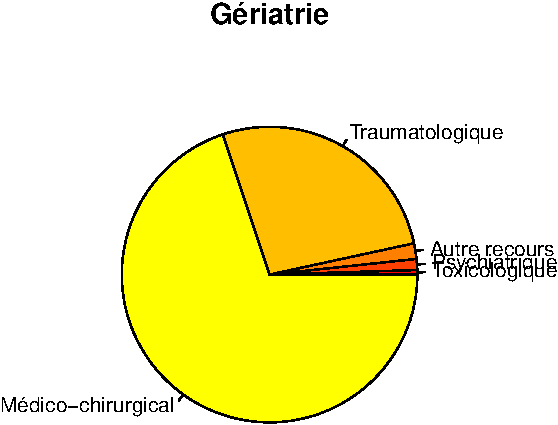
\includegraphics{analyse_merge_files/figure-latex/geriatrie-1.pdf}\\

\begin{Shaded}
\begin{Highlighting}[]
\NormalTok{tabp <-}\StringTok{ }\KeywordTok{tab1}\NormalTok{(d3g$TYPE_URGENCES, }\DataTypeTok{sort.group =} \StringTok{"decreasing"}\NormalTok{, }\DataTypeTok{bar.values =} \StringTok{"percent"}\NormalTok{, }\DataTypeTok{cex.names =} \FloatTok{0.8}\NormalTok{, }\DataTypeTok{main =} \KeywordTok{paste0}\NormalTok{(}\StringTok{"Médico-chirurgical gériatrique (N = "}\NormalTok{, n.ger, }\StringTok{")"}\NormalTok{), }\DataTypeTok{missing =} \OtherTok{FALSE}\NormalTok{)}
\end{Highlighting}
\end{Shaded}

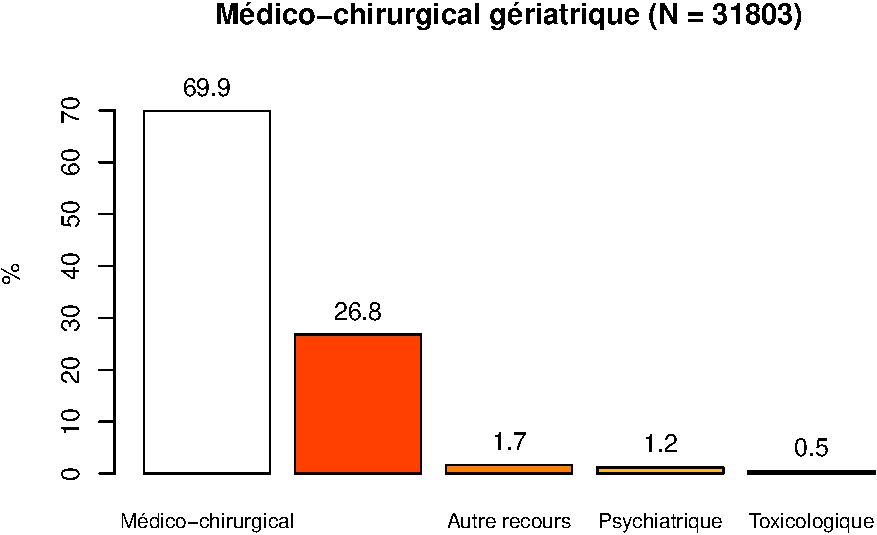
\includegraphics{analyse_merge_files/figure-latex/geriatrie-2.pdf}\\
Synthèse --------

\begin{Shaded}
\begin{Highlighting}[]
\CommentTok{# table de regroupement}
\NormalTok{t.type <-}\StringTok{ }\KeywordTok{rbind}\NormalTok{(s.type.adl, s.type.ped, s.type.ger)}
\NormalTok{t.type}
\end{Highlighting}
\end{Shaded}

\begin{verbatim}
##            Autre recours Médico-chirurgical Psychiatrique Toxicologique
## s.type.adl          6298              95992          5423          4167
## s.type.ped          2559              54620           924           547
## s.type.ger           643              26405           454           186
##            Traumatologique
## s.type.adl           62025
## s.type.ped           44213
## s.type.ger           10096
\end{verbatim}

\begin{Shaded}
\begin{Highlighting}[]
\KeywordTok{barplot}\NormalTok{(t.type)}
\end{Highlighting}
\end{Shaded}

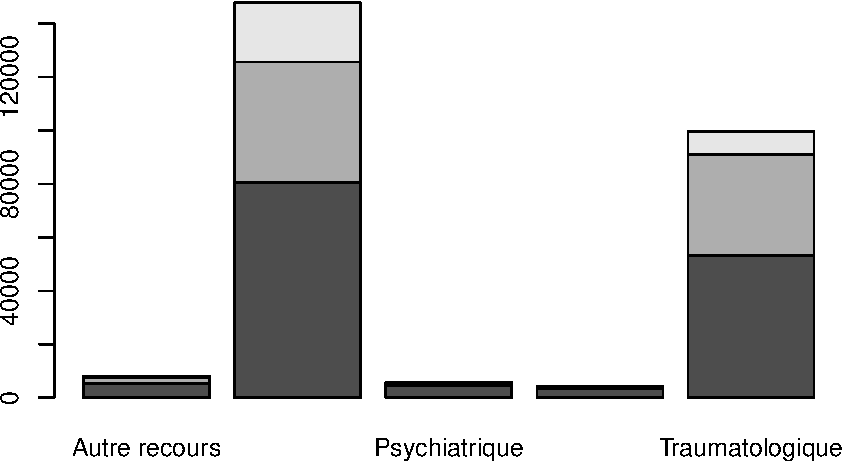
\includegraphics{analyse_merge_files/figure-latex/synthese-1.pdf}\\

\begin{Shaded}
\begin{Highlighting}[]
\CommentTok{# en pourcentages}
\NormalTok{p.type <-}\StringTok{ }\KeywordTok{round}\NormalTok{(}\KeywordTok{prop.table}\NormalTok{(t.type, }\DataTypeTok{margin =} \DecValTok{1}\NormalTok{)*}\DecValTok{100}\NormalTok{, }\DecValTok{2}\NormalTok{)}
\NormalTok{p.type}
\end{Highlighting}
\end{Shaded}

\begin{verbatim}
##            Autre recours Médico-chirurgical Psychiatrique Toxicologique
## s.type.adl          3.62              55.20          3.12          2.40
## s.type.ped          2.49              53.10          0.90          0.53
## s.type.ger          1.70              69.88          1.20          0.49
##            Traumatologique
## s.type.adl           35.67
## s.type.ped           42.98
## s.type.ger           26.72
\end{verbatim}

\begin{Shaded}
\begin{Highlighting}[]
\NormalTok{color <-}\StringTok{ }\KeywordTok{c}\NormalTok{(}\StringTok{"red"}\NormalTok{, }\StringTok{"green"}\NormalTok{, }\StringTok{"yellow"}\NormalTok{)}
\KeywordTok{barplot}\NormalTok{(p.type, }\DataTypeTok{cex.names =} \FloatTok{0.6}\NormalTok{)}
\end{Highlighting}
\end{Shaded}

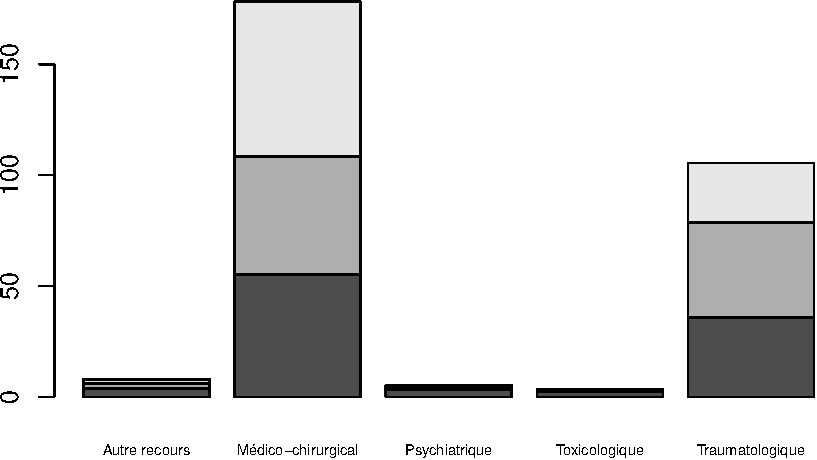
\includegraphics{analyse_merge_files/figure-latex/synthese-2.pdf}\\

\begin{Shaded}
\begin{Highlighting}[]
\KeywordTok{barplot}\NormalTok{(p.type, }\DataTypeTok{cex.names =} \FloatTok{0.6}\NormalTok{, }\DataTypeTok{beside =} \OtherTok{TRUE}\NormalTok{, }\DataTypeTok{col =} \NormalTok{color, }\DataTypeTok{main =} \StringTok{"Pathologies selon l'age"}\NormalTok{)}
\KeywordTok{legend}\NormalTok{(}\StringTok{"topright"}\NormalTok{, }\DataTypeTok{legend =} \KeywordTok{c}\NormalTok{(}\StringTok{"18-75 ans"}\NormalTok{,}\StringTok{"0-18 ans"}\NormalTok{,}\StringTok{"Sup.75 ans"}\NormalTok{), }\DataTypeTok{col =} \NormalTok{color, }\DataTypeTok{pch =} \DecValTok{15}\NormalTok{)}
\end{Highlighting}
\end{Shaded}

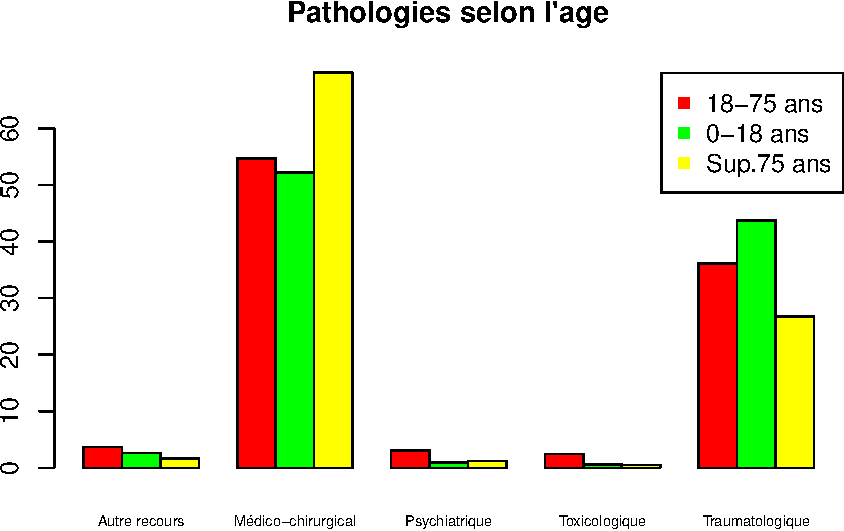
\includegraphics{analyse_merge_files/figure-latex/synthese-3.pdf}\\ Par
chapitre ============

\subsection{Adultes}\label{adultes}

\subsubsection{Pathologie
médico-chirurgicale}\label{pathologie-medico-chirurgicale}

\begin{Shaded}
\begin{Highlighting}[]
\NormalTok{medic.adl <-}\StringTok{ }\NormalTok{d3a[d3a$TYPE_URGENCES ==}\StringTok{ "Médico-chirurgical"}\NormalTok{,]}
\NormalTok{n.medic.adl <-}\StringTok{ }\KeywordTok{nrow}\NormalTok{(medic.adl)}
\NormalTok{s.medic.adl <-}\StringTok{ }\KeywordTok{table}\NormalTok{(}\KeywordTok{factor}\NormalTok{(medic.adl$CHAPITRE))}
\NormalTok{p.medic.adl <-}\StringTok{ }\KeywordTok{round}\NormalTok{(}\KeywordTok{prop.table}\NormalTok{(s.medic.adl)*}\DecValTok{100}\NormalTok{, }\DecValTok{2}\NormalTok{)}
\KeywordTok{sort}\NormalTok{(p.medic.adl, }\DataTypeTok{decreasing =} \OtherTok{TRUE}\NormalTok{)}
\end{Highlighting}
\end{Shaded}

\begin{verbatim}
## 
##            Douleurs de membre, rhumatologie, orthopédie, SNP 
##                                                        18.77 
##                 Douleurs abdominales, pathologies digestives 
##                                                        17.42 
##            ORL, ophtalmo, stomato et carrefour aéro-digestif 
##                                                         9.72 
##               Douleurs pelviennes, pathologies uro-génitales 
##                                                         9.34 
##         Douleurs thoraciques, pathologies cardio-vasculaires 
##                                                         8.83 
##                Céphalées, pathologies neurologiques hors SNP 
##                                                         7.78 
##          Dermato-allergologie et atteintes cutanéo-muqueuses 
##                                                         6.99 
##                        Signes généraux et autres pathologies 
##                                                         6.37 
## Malaises, lipothymies, syncopes, étourdissements et vertiges 
##                                                         6.21 
##        Dyspnées, pathologies des voies aériennes inférieures 
##                                                         6.19 
##                             Fièvre et infectiologie générale 
##                                                         2.38
\end{verbatim}

\begin{Shaded}
\begin{Highlighting}[]
\KeywordTok{tab1}\NormalTok{(}\KeywordTok{factor}\NormalTok{(medic.adl$CHAPITRE), }\DataTypeTok{cex.names =} \FloatTok{0.5}\NormalTok{, }\DataTypeTok{cex =} \FloatTok{0.8}\NormalTok{, }\DataTypeTok{sort.group =} \StringTok{"decreasing"}\NormalTok{, }\DataTypeTok{main =} \StringTok{"Médico-chir adultes"}\NormalTok{, }\DataTypeTok{bar.values =} \StringTok{"percent"}\NormalTok{)}
\end{Highlighting}
\end{Shaded}

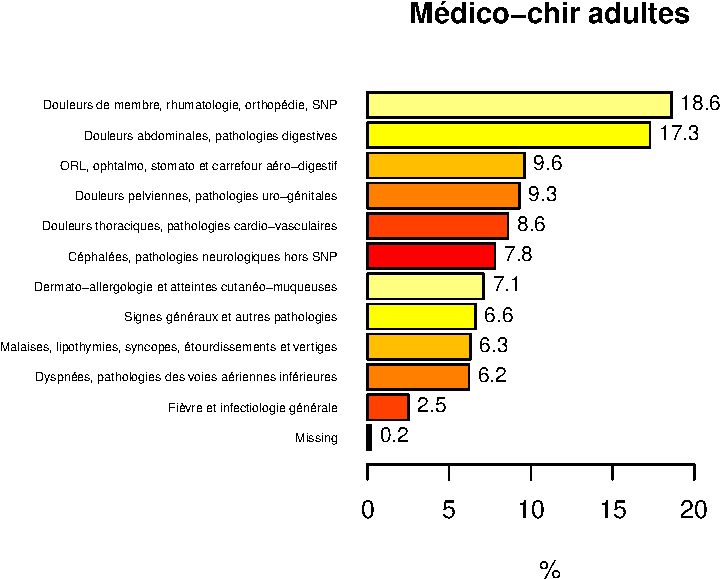
\includegraphics{analyse_merge_files/figure-latex/chap_adultes-1.pdf}\\

\begin{verbatim}
## factor(medic.adl$CHAPITRE) : 
##                                                              Frequency
## Douleurs de membre, rhumatologie, orthopédie, SNP                18021
## Douleurs abdominales, pathologies digestives                     16725
## ORL, ophtalmo, stomato et carrefour aéro-digestif                 9326
## Douleurs pelviennes, pathologies uro-génitales                    8965
## Douleurs thoraciques, pathologies cardio-vasculaires              8474
## Céphalées, pathologies neurologiques hors SNP                     7466
## Dermato-allergologie et atteintes cutanéo-muqueuses               6708
## Signes généraux et autres pathologies                             6119
## Malaises, lipothymies, syncopes, étourdissements et vertiges      5959
## Dyspnées, pathologies des voies aériennes inférieures             5945
## Fièvre et infectiologie générale                                  2284
## NA's                                                               220
##   Total                                                          96212
##                                                                %(NA+)
## Douleurs de membre, rhumatologie, orthopédie, SNP                18.7
## Douleurs abdominales, pathologies digestives                     17.4
## ORL, ophtalmo, stomato et carrefour aéro-digestif                 9.7
## Douleurs pelviennes, pathologies uro-génitales                    9.3
## Douleurs thoraciques, pathologies cardio-vasculaires              8.8
## Céphalées, pathologies neurologiques hors SNP                     7.8
## Dermato-allergologie et atteintes cutanéo-muqueuses               7.0
## Signes généraux et autres pathologies                             6.4
## Malaises, lipothymies, syncopes, étourdissements et vertiges      6.2
## Dyspnées, pathologies des voies aériennes inférieures             6.2
## Fièvre et infectiologie générale                                  2.4
## NA's                                                              0.2
##   Total                                                         100.0
##                                                                %(NA-)
## Douleurs de membre, rhumatologie, orthopédie, SNP                18.8
## Douleurs abdominales, pathologies digestives                     17.4
## ORL, ophtalmo, stomato et carrefour aéro-digestif                 9.7
## Douleurs pelviennes, pathologies uro-génitales                    9.3
## Douleurs thoraciques, pathologies cardio-vasculaires              8.8
## Céphalées, pathologies neurologiques hors SNP                     7.8
## Dermato-allergologie et atteintes cutanéo-muqueuses               7.0
## Signes généraux et autres pathologies                             6.4
## Malaises, lipothymies, syncopes, étourdissements et vertiges      6.2
## Dyspnées, pathologies des voies aériennes inférieures             6.2
## Fièvre et infectiologie générale                                  2.4
## NA's                                                              0.0
##   Total                                                         100.0
\end{verbatim}

\subsubsection{Pathologie traumatique}\label{pathologie-traumatique}

\begin{Shaded}
\begin{Highlighting}[]
\NormalTok{trauma.adl <-}\StringTok{ }\NormalTok{d3a[d3a$TYPE_URGENCES ==}\StringTok{ "Traumatologique"}\NormalTok{,]}
\NormalTok{n.trauma.adl <-}\StringTok{ }\KeywordTok{nrow}\NormalTok{(trauma.adl)}
\NormalTok{s.trauma.adl <-}\StringTok{ }\KeywordTok{table}\NormalTok{(}\KeywordTok{factor}\NormalTok{(trauma.adl$CHAPITRE))}
\NormalTok{p.trauma.adl <-}\StringTok{ }\KeywordTok{round}\NormalTok{(}\KeywordTok{prop.table}\NormalTok{(s.trauma.adl)*}\DecValTok{100}\NormalTok{, }\DecValTok{2}\NormalTok{)}
\KeywordTok{sort}\NormalTok{(p.trauma.adl, }\DataTypeTok{decreasing =} \OtherTok{TRUE}\NormalTok{)}
\end{Highlighting}
\end{Shaded}

\begin{verbatim}
## 
##      Traumatisme du membre supérieur      Traumatisme du membre inférieur 
##                                37.38                                31.11 
##     Traumatisme de la tête et du cou Traumatisme thoraco-abdomino-pelvien 
##                                17.18                                 7.20 
##  Traumatisme autre et sans précision 
##                                 7.14
\end{verbatim}

\begin{Shaded}
\begin{Highlighting}[]
\KeywordTok{tab1}\NormalTok{(}\KeywordTok{factor}\NormalTok{(trauma.adl$CHAPITRE), }\DataTypeTok{cex.names =} \FloatTok{0.5}\NormalTok{, }\DataTypeTok{cex =} \FloatTok{0.8}\NormalTok{, }\DataTypeTok{sort.group =} \StringTok{"decreasing"}\NormalTok{, }\DataTypeTok{main =} \StringTok{"Traumatologie adultes"}\NormalTok{, }\DataTypeTok{bar.values =} \StringTok{"percent"}\NormalTok{, }\DataTypeTok{horiz =} \OtherTok{TRUE}\NormalTok{)}
\end{Highlighting}
\end{Shaded}

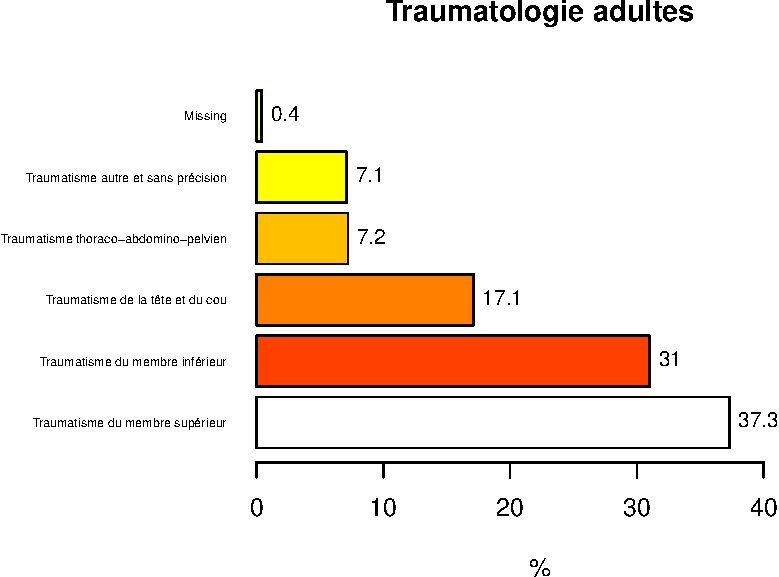
\includegraphics{analyse_merge_files/figure-latex/trauma_adulte-1.pdf}\\

\begin{verbatim}
## factor(trauma.adl$CHAPITRE) : 
##                                      Frequency   %(NA+)   %(NA-)
## Traumatisme du membre supérieur          23188     37.3     37.4
## Traumatisme du membre inférieur          19293     31.0     31.1
## Traumatisme de la tête et du cou         10653     17.1     17.2
## Traumatisme thoraco-abdomino-pelvien      4464      7.2      7.2
## Traumatisme autre et sans précision       4427      7.1      7.1
## NA's                                       220      0.4      0.0
##   Total                                  62245    100.0    100.0
\end{verbatim}

\subsection{Enfants}\label{enfants}

\subsubsection{Pathologie médico-chirurgicale
pédiatrique}\label{pathologie-medico-chirurgicale-pediatrique}

\begin{Shaded}
\begin{Highlighting}[]
\NormalTok{f <-}\StringTok{ }\KeywordTok{groupe.pathologique}\NormalTok{(d3p, }\StringTok{"medchir"}\NormalTok{)}
\KeywordTok{tab1}\NormalTok{(f$data, }\DataTypeTok{cex.names =} \FloatTok{0.5}\NormalTok{, }\DataTypeTok{cex =} \FloatTok{0.8}\NormalTok{, }\DataTypeTok{sort.group =} \StringTok{"decreasing"}\NormalTok{, }\DataTypeTok{main =} \StringTok{"Médico-chir pédiatrique"}\NormalTok{, }\DataTypeTok{bar.values =} \StringTok{"percent"}\NormalTok{)}
\end{Highlighting}
\end{Shaded}

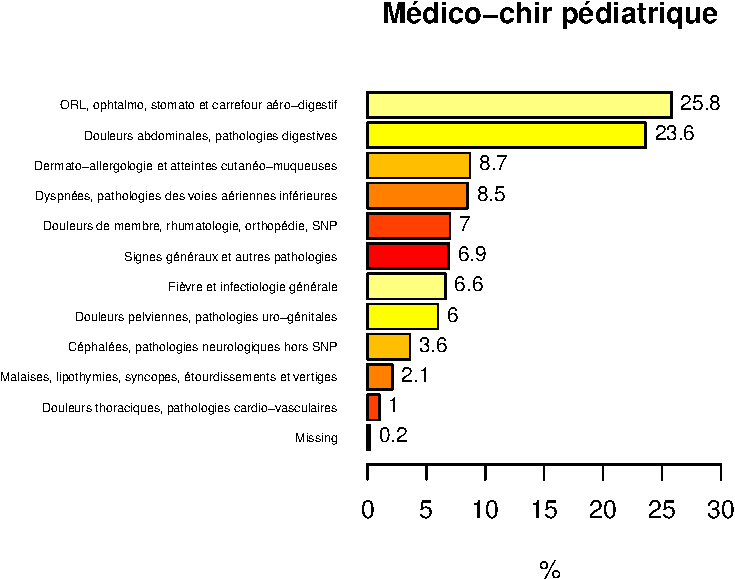
\includegraphics{analyse_merge_files/figure-latex/chap_ped_med-1.pdf}\\

\begin{verbatim}
## f$data : 
##                                                              Frequency
## ORL, ophtalmo, stomato et carrefour aéro-digestif                14093
## Douleurs abdominales, pathologies digestives                     12906
## Dermato-allergologie et atteintes cutanéo-muqueuses               4770
## Dyspnées, pathologies des voies aériennes inférieures             4644
## Douleurs de membre, rhumatologie, orthopédie, SNP                 3857
## Signes généraux et autres pathologies                             3788
## Fièvre et infectiologie générale                                  3601
## Douleurs pelviennes, pathologies uro-génitales                    3295
## Céphalées, pathologies neurologiques hors SNP                     1994
## Malaises, lipothymies, syncopes, étourdissements et vertiges      1132
## Douleurs thoraciques, pathologies cardio-vasculaires               540
## NA's                                                               100
##   Total                                                          54720
##                                                                %(NA+)
## ORL, ophtalmo, stomato et carrefour aéro-digestif                25.8
## Douleurs abdominales, pathologies digestives                     23.6
## Dermato-allergologie et atteintes cutanéo-muqueuses               8.7
## Dyspnées, pathologies des voies aériennes inférieures             8.5
## Douleurs de membre, rhumatologie, orthopédie, SNP                 7.0
## Signes généraux et autres pathologies                             6.9
## Fièvre et infectiologie générale                                  6.6
## Douleurs pelviennes, pathologies uro-génitales                    6.0
## Céphalées, pathologies neurologiques hors SNP                     3.6
## Malaises, lipothymies, syncopes, étourdissements et vertiges      2.1
## Douleurs thoraciques, pathologies cardio-vasculaires              1.0
## NA's                                                              0.2
##   Total                                                         100.0
##                                                                %(NA-)
## ORL, ophtalmo, stomato et carrefour aéro-digestif                25.8
## Douleurs abdominales, pathologies digestives                     23.6
## Dermato-allergologie et atteintes cutanéo-muqueuses               8.7
## Dyspnées, pathologies des voies aériennes inférieures             8.5
## Douleurs de membre, rhumatologie, orthopédie, SNP                 7.1
## Signes généraux et autres pathologies                             6.9
## Fièvre et infectiologie générale                                  6.6
## Douleurs pelviennes, pathologies uro-génitales                    6.0
## Céphalées, pathologies neurologiques hors SNP                     3.7
## Malaises, lipothymies, syncopes, étourdissements et vertiges      2.1
## Douleurs thoraciques, pathologies cardio-vasculaires              1.0
## NA's                                                              0.0
##   Total                                                         100.0
\end{verbatim}

\subsubsection{Pathologie traumatique
pédiatrique}\label{pathologie-traumatique-pediatrique}

\begin{Shaded}
\begin{Highlighting}[]
\NormalTok{f <-}\StringTok{ }\KeywordTok{groupe.pathologique}\NormalTok{(d3p, }\StringTok{"trau"}\NormalTok{)}
\KeywordTok{tab1}\NormalTok{(f$data, }\DataTypeTok{cex.names =} \FloatTok{0.5}\NormalTok{, }\DataTypeTok{cex =} \FloatTok{0.8}\NormalTok{, }\DataTypeTok{sort.group =} \StringTok{"decreasing"}\NormalTok{, }\DataTypeTok{main =} \StringTok{"Traumatologie pédiatrique"}\NormalTok{, }\DataTypeTok{bar.values =} \StringTok{"percent"}\NormalTok{)}
\end{Highlighting}
\end{Shaded}

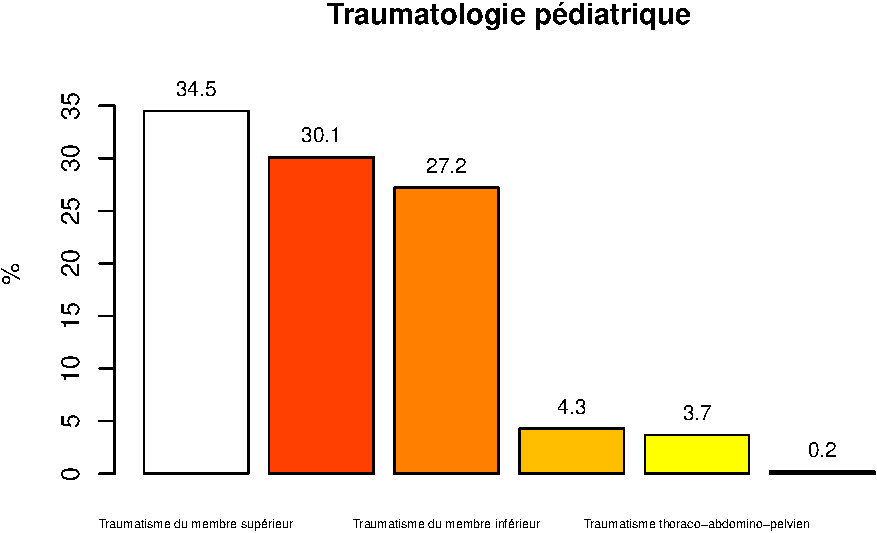
\includegraphics{analyse_merge_files/figure-latex/chap_ped_trau-1.pdf}\\

\begin{verbatim}
## f$data : 
##                                      Frequency   %(NA+)   %(NA-)
## Traumatisme du membre supérieur          15182     34.3     34.3
## Traumatisme de la tête et du cou         13401     30.2     30.3
## Traumatisme du membre inférieur          12126     27.4     27.4
## Traumatisme autre et sans précision       1864      4.2      4.2
## Traumatisme thoraco-abdomino-pelvien      1640      3.7      3.7
## NA's                                       100      0.2      0.0
##   Total                                  44313    100.0    100.0
\end{verbatim}

\subsection{Gériatrie}\label{geriatrie}

\subsubsection{Pathologie médico-chirurgicale
gériatrique}\label{pathologie-medico-chirurgicale-geriatrique}

\begin{Shaded}
\begin{Highlighting}[]
\NormalTok{f <-}\StringTok{ }\KeywordTok{groupe.pathologique}\NormalTok{(d3g, }\StringTok{"medchir"}\NormalTok{)}
\KeywordTok{tab1}\NormalTok{(f$data, }\DataTypeTok{cex.names =} \FloatTok{0.5}\NormalTok{, }\DataTypeTok{cex =} \FloatTok{0.8}\NormalTok{, }\DataTypeTok{sort.group =} \StringTok{"decreasing"}\NormalTok{, }\DataTypeTok{main =} \StringTok{"Médico-chir gériatrique"}\NormalTok{, }\DataTypeTok{bar.values =} \StringTok{"percent"}\NormalTok{)}
\end{Highlighting}
\end{Shaded}

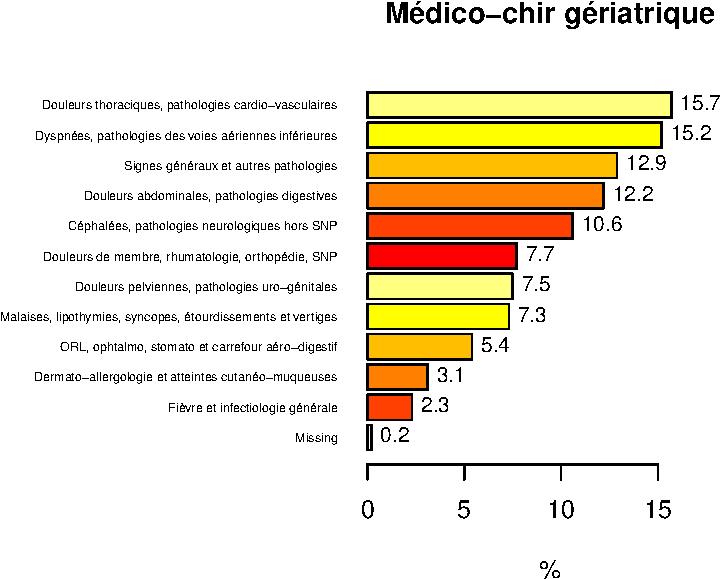
\includegraphics{analyse_merge_files/figure-latex/chap_ger_med-1.pdf}\\

\begin{verbatim}
## f$data : 
##                                                              Frequency
## Douleurs thoraciques, pathologies cardio-vasculaires              4165
## Dyspnées, pathologies des voies aériennes inférieures             4032
## Signes généraux et autres pathologies                             3407
## Douleurs abdominales, pathologies digestives                      3218
## Céphalées, pathologies neurologiques hors SNP                     2796
## Douleurs de membre, rhumatologie, orthopédie, SNP                 2033
## Douleurs pelviennes, pathologies uro-génitales                    1979
## Malaises, lipothymies, syncopes, étourdissements et vertiges      1936
## ORL, ophtalmo, stomato et carrefour aéro-digestif                 1427
## Dermato-allergologie et atteintes cutanéo-muqueuses                808
## Fièvre et infectiologie générale                                   604
## NA's                                                                45
##   Total                                                          26450
##                                                                %(NA+)
## Douleurs thoraciques, pathologies cardio-vasculaires             15.7
## Dyspnées, pathologies des voies aériennes inférieures            15.2
## Signes généraux et autres pathologies                            12.9
## Douleurs abdominales, pathologies digestives                     12.2
## Céphalées, pathologies neurologiques hors SNP                    10.6
## Douleurs de membre, rhumatologie, orthopédie, SNP                 7.7
## Douleurs pelviennes, pathologies uro-génitales                    7.5
## Malaises, lipothymies, syncopes, étourdissements et vertiges      7.3
## ORL, ophtalmo, stomato et carrefour aéro-digestif                 5.4
## Dermato-allergologie et atteintes cutanéo-muqueuses               3.1
## Fièvre et infectiologie générale                                  2.3
## NA's                                                              0.2
##   Total                                                         100.0
##                                                                %(NA-)
## Douleurs thoraciques, pathologies cardio-vasculaires             15.8
## Dyspnées, pathologies des voies aériennes inférieures            15.3
## Signes généraux et autres pathologies                            12.9
## Douleurs abdominales, pathologies digestives                     12.2
## Céphalées, pathologies neurologiques hors SNP                    10.6
## Douleurs de membre, rhumatologie, orthopédie, SNP                 7.7
## Douleurs pelviennes, pathologies uro-génitales                    7.5
## Malaises, lipothymies, syncopes, étourdissements et vertiges      7.3
## ORL, ophtalmo, stomato et carrefour aéro-digestif                 5.4
## Dermato-allergologie et atteintes cutanéo-muqueuses               3.1
## Fièvre et infectiologie générale                                  2.3
## NA's                                                              0.0
##   Total                                                         100.0
\end{verbatim}

\subsubsection{Pathologie traumatique
gériatrique}\label{pathologie-traumatique-geriatrique}

\begin{Shaded}
\begin{Highlighting}[]
\NormalTok{f <-}\StringTok{ }\KeywordTok{groupe.pathologique}\NormalTok{(d3g, }\StringTok{"trau"}\NormalTok{)}
\KeywordTok{tab1}\NormalTok{(f$data, }\DataTypeTok{cex.names =} \FloatTok{0.5}\NormalTok{, }\DataTypeTok{cex =} \FloatTok{0.8}\NormalTok{, }\DataTypeTok{sort.group =} \StringTok{"decreasing"}\NormalTok{, }\DataTypeTok{main =} \StringTok{"Traumatologie gériatrique"}\NormalTok{, }\DataTypeTok{bar.values =} \StringTok{"percent"}\NormalTok{)}
\end{Highlighting}
\end{Shaded}

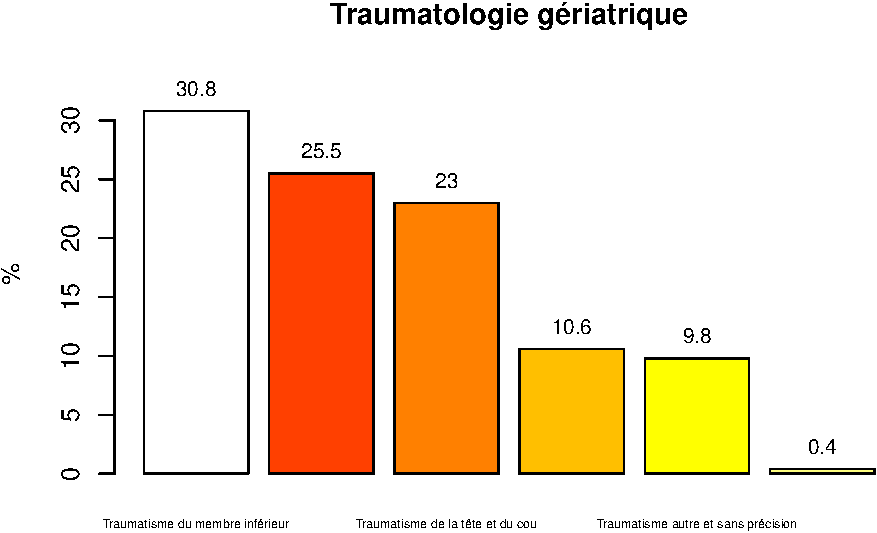
\includegraphics{analyse_merge_files/figure-latex/chap_ger_trau-1.pdf}\\

\begin{verbatim}
## f$data : 
##                                      Frequency   %(NA+)   %(NA-)
## Traumatisme du membre inférieur           3110     30.7     30.8
## Traumatisme du membre supérieur           2544     25.1     25.2
## Traumatisme de la tête et du cou          2353     23.2     23.3
## Traumatisme thoraco-abdomino-pelvien      1085     10.7     10.7
## Traumatisme autre et sans précision       1004      9.9      9.9
## NA's                                        45      0.4      0.0
##   Total                                  10141    100.0    100.0
\end{verbatim}

\subsection{Synthèse}\label{synthese}

Passages bruts:

\begin{verbatim}
Warning in rbind(s.type.ped, s.type.adl, s.type.ger, s.type): number of
columns of result is not a multiple of vector length (arg 1)
\end{verbatim}

\begin{verbatim}
               Autre recours Médico-chirurgical Psychiatrique
< 18 ans                2559              54620           924
18-74 ans               6298              95992          5423
75 ans et plus           643              26405           454
TOTAL                   9500             177017          6803
               Toxicologique Traumatologique NA's
< 18 ans                 547           44213 2559
18-74 ans               4167           62025 6298
75 ans et plus           186           10096  643
TOTAL                   4900          116334  359
\end{verbatim}

Taux de passage standardisé pour 1000 RPU:

\begin{verbatim}
Warning in rbind(t1, t2, t3, t4): number of columns of result is not a
multiple of vector length (arg 1)
\end{verbatim}

\begin{verbatim}
               Autre recours Médico-chirurgical Psychiatrique
< 18 ans               24.88             531.00          8.98
18-74 ans              36.22             551.98         31.18
75 ans et plus         17.02             698.84         12.02
TOTAL                  30.17             562.11         21.60
               Toxicologique Traumatologique  NA's
< 18 ans                5.32          429.82 24.88
18-74 ans              23.96          356.66 36.22
75 ans et plus          4.92          267.20 17.02
TOTAL                  15.56          369.42  1.14
\end{verbatim}

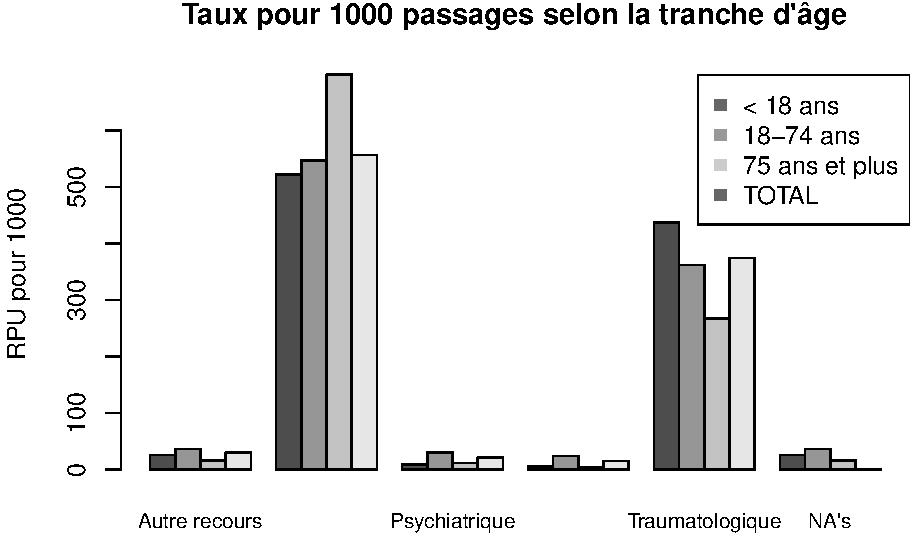
\includegraphics{analyse_merge_files/figure-latex/synthese2-1.pdf}\\

\section{AVC}\label{avc}

\begin{Shaded}
\begin{Highlighting}[]
\NormalTok{AVC<-d3[}\KeywordTok{substr}\NormalTok{(d3$DP,}\DecValTok{1}\NormalTok{,}\DecValTok{3}\NormalTok{)>=}\StringTok{"I60"} \NormalTok{&}\StringTok{ }\KeywordTok{substr}\NormalTok{(d3$DP,}\DecValTok{1}\NormalTok{,}\DecValTok{3}\NormalTok{)<}\StringTok{"I65"} \NormalTok{|}\StringTok{ }\KeywordTok{substr}\NormalTok{(d3$DP,}\DecValTok{1}\NormalTok{,}\DecValTok{3}\NormalTok{)==}\StringTok{"G46"} \NormalTok{|}\StringTok{ }\KeywordTok{substr}\NormalTok{(d3$DP,}\DecValTok{1}\NormalTok{,}\DecValTok{3}\NormalTok{)==}\StringTok{"G45"} \NormalTok{,]}
\NormalTok{AVC$etiologie <-}\StringTok{ }\OtherTok{NA}
\NormalTok{AVC$etiologie[}\KeywordTok{substr}\NormalTok{(AVC$DP,}\DecValTok{1}\NormalTok{,}\DecValTok{3}\NormalTok{) %in%}\StringTok{ }\KeywordTok{c}\NormalTok{(}\StringTok{"I60"}\NormalTok{,}\StringTok{"I61"}\NormalTok{,}\StringTok{"I62"}\NormalTok{)] <-}\StringTok{"HEMO"}
\NormalTok{AVC$etiologie[}\KeywordTok{substr}\NormalTok{(AVC$DP,}\DecValTok{1}\NormalTok{,}\DecValTok{3}\NormalTok{) %in%}\StringTok{ }\KeywordTok{c}\NormalTok{(}\StringTok{"I63"}\NormalTok{,}\StringTok{"I64"}\NormalTok{)] <-}\StringTok{"ISCH"}
\NormalTok{AVC$etiologie[}\KeywordTok{substr}\NormalTok{(AVC$DP,}\DecValTok{1}\NormalTok{,}\DecValTok{3}\NormalTok{) %in%}\StringTok{ }\KeywordTok{c}\NormalTok{(}\StringTok{"I64"}\NormalTok{)] <-}\StringTok{"NPRE"}
\NormalTok{AVC$etiologie[}\KeywordTok{substr}\NormalTok{(AVC$DP,}\DecValTok{1}\NormalTok{,}\DecValTok{3}\NormalTok{) %in%}\StringTok{ }\KeywordTok{c}\NormalTok{(}\StringTok{"G45"}\NormalTok{,}\StringTok{"G46"}\NormalTok{)] <-}\StringTok{"AIT"}
\NormalTok{AVC$etiologie <-}\StringTok{ }\KeywordTok{as.factor}\NormalTok{(AVC$etiologie)}

\NormalTok{n.avc <-}\StringTok{ }\KeywordTok{nrow}\NormalTok{(AVC)}
\end{Highlighting}
\end{Shaded}

\subsection{RECUEIL DES DONNÉES}\label{recueil-des-donnees}

\begin{itemize}
\itemsep1pt\parskip0pt\parsep0pt
\item
  Nombre d'AVC dans l'année (+ rappeler le pourcentage d'exhaustivité du
  DP par rapport au nombre de RPU): \textbf{2945}
\item
  Moyenne quotidienne d'AVC: \textbf{8.0684932 AVC/j}
\item
  \% d'AVC dans l'activité globale: \textbf{0.9351789 \%}
\end{itemize}

\subsection{PATIENTS}\label{patients}

\begin{verbatim}
## c.age
##     [0,5)    [5,10)   [10,15)   [15,20)   [20,25)   [25,30)   [30,35) 
##         5         6         1         8        24        20        30 
##   [35,40)   [40,45)   [45,50)   [50,55)   [55,60)   [60,65)   [65,70) 
##        40        59       108       137       170       238       284 
##   [70,75)   [75,80)   [80,85)   [85,90)   [90,95)  [95,100) [100,105) 
##       269       420       479       406       200        34         6 
## [105,110) [110,115) [115,120) 
##         1         0         0
\end{verbatim}

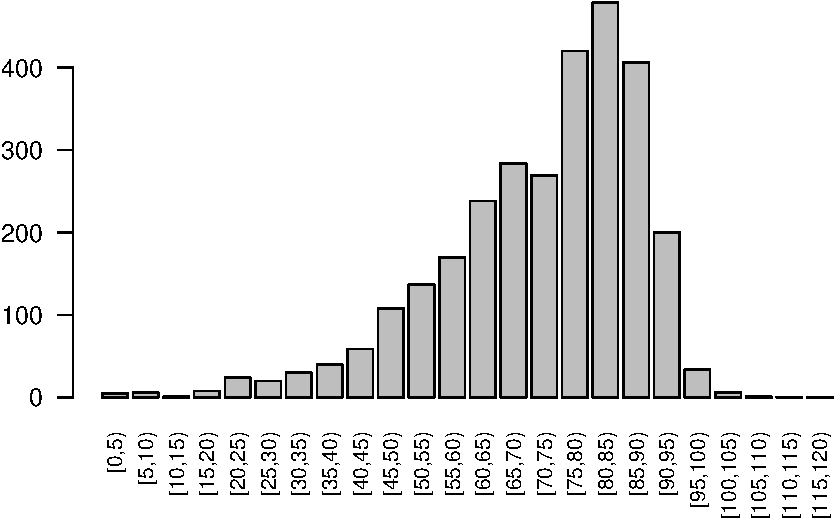
\includegraphics{analyse_merge_files/figure-latex/patients-1.pdf}\\ -
Sex ratio: 1.0020394 - Age moyen: 71.53 ans - Nombre d'AVC par sous
classe d'âge (GT1):

\subsection{ARRIVÉE}\label{arrivee}

\begin{itemize}
\itemsep1pt\parskip0pt\parsep0pt
\item
  Nombre d'AVC et \% par tranche d'heure GT1 (matinée, début d'après
  midi, fin d'après midi, soirée, nuit profonde)
\end{itemize}

\begin{Shaded}
\begin{Highlighting}[]
\CommentTok{# heures de découpage}
\NormalTok{p <-}\StringTok{ }\KeywordTok{c}\NormalTok{(}\DecValTok{0}\NormalTok{, }\DecValTok{8}\NormalTok{, }\DecValTok{12}\NormalTok{, }\DecValTok{16}\NormalTok{, }\DecValTok{20}\NormalTok{, }\DecValTok{24}\NormalTok{)}
\CommentTok{# légende}
\NormalTok{np <-}\StringTok{ }\KeywordTok{c}\NormalTok{(}\StringTok{"nuit profonde"}\NormalTok{, }\StringTok{"matinée"}\NormalTok{, }\StringTok{"début après-midi"}\NormalTok{, }\StringTok{"fin après-midi"}\NormalTok{, }\StringTok{"soirée"}\NormalTok{)}
\CommentTok{# extraction des heures à partir du format datetime (http://stackoverflow.com/questions/19292438/split-date-time)}
\NormalTok{a <-}\StringTok{ }\KeywordTok{as.numeric}\NormalTok{(}\KeywordTok{format}\NormalTok{(}\KeywordTok{as.POSIXct}\NormalTok{(AVC$ENTREE), }\StringTok{"%H"}\NormalTok{))}

\NormalTok{x <-}\StringTok{ }\KeywordTok{cut}\NormalTok{(a, p, np, }\DataTypeTok{right =} \OtherTok{FALSE}\NormalTok{)}
\NormalTok{x2 <-}\StringTok{ }\KeywordTok{cut}\NormalTok{(a, p, }\DataTypeTok{right =} \OtherTok{FALSE}\NormalTok{)}

\KeywordTok{rbind}\NormalTok{(}\KeywordTok{levels}\NormalTok{(x2), }\KeywordTok{table}\NormalTok{(x))}
\end{Highlighting}
\end{Shaded}

\begin{verbatim}
##      nuit profonde matinée  début après-midi fin après-midi soirée   
## [1,] "[0,8)"       "[8,12)" "[12,16)"        "[16,20)"      "[20,24)"
## [2,] "268"         "930"    "929"            "599"          "219"
\end{verbatim}

\begin{Shaded}
\begin{Highlighting}[]
\KeywordTok{tab1}\NormalTok{(x, }\DataTypeTok{cex.names =} \FloatTok{0.8}\NormalTok{, }\DataTypeTok{main =} \StringTok{"Heure d'admission des AVC"}\NormalTok{, }\DataTypeTok{bar.values =} \StringTok{"percent"}\NormalTok{, }\DataTypeTok{ylab =} \StringTok{"%"}\NormalTok{)}
\end{Highlighting}
\end{Shaded}

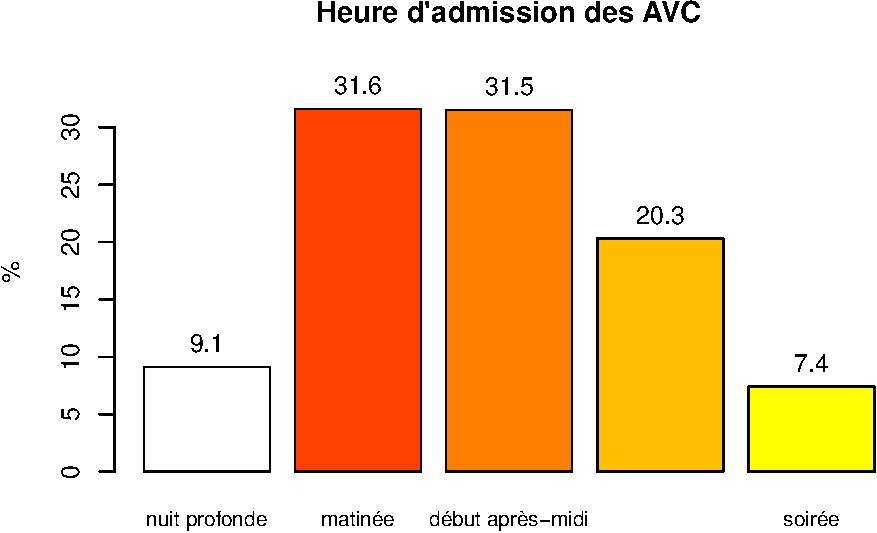
\includegraphics{analyse_merge_files/figure-latex/avc_periode-1.pdf}\\

\begin{verbatim}
## x : 
##                  Frequency Percent Cum. percent
## nuit profonde          268     9.1          9.1
## matinée                930    31.6         40.7
## début après-midi       929    31.5         72.2
## fin après-midi         599    20.3         92.6
## soirée                 219     7.4        100.0
##   Total               2945   100.0        100.0
\end{verbatim}

\begin{itemize}
\itemsep1pt\parskip0pt\parsep0pt
\item
  \% passages en horaire de PDS
\end{itemize}

PDSS = horaires de PDS en semaine, PDSWE = horaires de PDS le WE, NPDS =
hors horaire de PDS.

\subsection{Mode d'arrivée aux
urgences}\label{mode-darrivee-aux-urgences}

\begin{Shaded}
\begin{Highlighting}[]
\NormalTok{n.avc.moyen <-}\StringTok{ }\KeywordTok{summary}\NormalTok{(}\KeywordTok{factor}\NormalTok{(AVC$TRANSPORT))}
\NormalTok{n.avc.moyen}
\end{Highlighting}
\end{Shaded}

\begin{verbatim}
##  AMBU    FO  HELI PERSO  SMUR  VSAB  NA's 
##  1384     1    18   645    70   484   343
\end{verbatim}

\begin{Shaded}
\begin{Highlighting}[]
\NormalTok{p.avc.moyen <-}\StringTok{ }\KeywordTok{round}\NormalTok{(}\KeywordTok{prop.table}\NormalTok{(n.avc.moyen)*}\DecValTok{100}\NormalTok{, }\DecValTok{2}\NormalTok{)}
\NormalTok{p.avc.moyen}
\end{Highlighting}
\end{Shaded}

\begin{verbatim}
##  AMBU    FO  HELI PERSO  SMUR  VSAB  NA's 
## 46.99  0.03  0.61 21.90  2.38 16.43 11.65
\end{verbatim}

\begin{itemize}
\itemsep1pt\parskip0pt\parsep0pt
\item
  \% d'arrivées Moyen perso
\item
  \% d'arrivées SMUR
\item
  \% d'arrivées VSAV
\item
  \% d'arrivées ambulance privée NB : commentaire possible pour
  expliquer que la somme des 4 pourcentages ci dessus ne fait pas 100 \%
\end{itemize}

\subsection{DIAGNOSTIC PRINCIPAL}\label{diagnostic-principal}

\texttt{r   t.diag \textless{}- table(AVC\$etiologie)   p.diag \textless{}- prop.table(t.diag)*100}

\begin{itemize}
\itemsep1pt\parskip0pt\parsep0pt
\item
  Nombre d'AVC et \%
\item
  Nombre d'AIT et \%
\item
  Nombre de codes ``symptomatiques'' (hémiplégie, aphasie, amaurose,
  etc\ldots{}) et \%
\item
  Nombre d'autres hémorragies non traumatiques et \%
\end{itemize}

NB : se référer à l'annexe 4 pour les regroupements.

\subsection{DURÉE}\label{duree}

\begin{itemize}
\itemsep1pt\parskip0pt\parsep0pt
\item
  Durée de passage (HORS UHCD) : moyenne et médiane
\item
  \% de passages de moins de 4h
\end{itemize}

\subsection{MODE DE SORTIE}\label{mode-de-sortie}

\begin{itemize}
\itemsep1pt\parskip0pt\parsep0pt
\item
  \% d'hospitalisation
\item
  \% de mutation
\item
  \% de transfert
\item
  \% de retour à domicile
\end{itemize}

\section{Résultats par type
d'établissement}\label{resultats-par-type-detablissement}

La trame commune recueuille les éléments suivants:

\begin{verbatim}
                 Autre recours Médico-chirurgical Psychiatrique
SU SAMU CHU              24.88                531          8.98
SU SAMU non CHU        1056.00              18671       1416.00
SU SMUR non SAMU       4972.00              75018       2880.00
SU non SMUR            2163.00              31674        575.00
TOTAL                  9500.00             177017       6803.00
                 Toxicologique Traumatologique
SU SAMU CHU               5.32          429.82
SU SAMU non CHU         696.00         7819.00
SU SMUR non SAMU       2217.00        55814.00
SU non SMUR             234.00        29147.00
TOTAL                  4900.00       116334.00
\end{verbatim}

Une table des types

\begin{Shaded}
\begin{Highlighting}[]
\NormalTok{x <-}\StringTok{ }\KeywordTok{tapply}\NormalTok{(d3$TYPE_URGENCES, d3$FINESS, table ) }\CommentTok{# x est un vecteur de list}
\NormalTok{y <-}\StringTok{ }\NormalTok{x[-}\DecValTok{3}\NormalTok{] }\CommentTok{# on retire ste anne qui n'a aucun DP}
\NormalTok{z <-}\StringTok{ }\KeywordTok{matrix}\NormalTok{(}\KeywordTok{unlist}\NormalTok{(y), }\DataTypeTok{nrow =} \KeywordTok{length}\NormalTok{(y), }\DataTypeTok{ncol =} \DecValTok{5}\NormalTok{) }\CommentTok{# on transforme y en matrice. Pour en faire un data frame: df <- df <- data.frame(matrix(unlist(y), nrow=14, byrow=T),stringsAsFactors=FALSE). Source: http://stackoverflow.com/questions/4227223/r-list-to-data-frame}
\end{Highlighting}
\end{Shaded}

\begin{verbatim}
## Warning in matrix(unlist(y), nrow = length(y), ncol = 5): la longueur des
## données [85] n'est pas un diviseur ni un multiple du nombre de lignes [19]
\end{verbatim}

\begin{Shaded}
\begin{Highlighting}[]
\KeywordTok{rownames}\NormalTok{(z) <-}\StringTok{ }\KeywordTok{names}\NormalTok{(x[-}\DecValTok{3}\NormalTok{]) }\CommentTok{# ok}
\KeywordTok{colnames}\NormalTok{(z) <-}\StringTok{ }\KeywordTok{names}\NormalTok{(}\KeywordTok{unlist}\NormalTok{(x[}\DecValTok{1}\NormalTok{])) }\CommentTok{# ok mais pas terrible}
\end{Highlighting}
\end{Shaded}

\section{Pathologies en UHTCD}\label{pathologies-en-uhtcd}

Qui sont les patients hospitalisés en UHTCD ?

\begin{Shaded}
\begin{Highlighting}[]
\NormalTok{dp.uhcd <-}\StringTok{ }\NormalTok{d3[d3$ORIENTATION ==}\StringTok{ "UHCD"}\NormalTok{,]}
\KeywordTok{summary}\NormalTok{(dp.uhcd$TYPE_URGENCES)}
\end{Highlighting}
\end{Shaded}

\begin{verbatim}
     Autre recours Médico-chirurgical      Psychiatrique 
               231              12784                360 
     Toxicologique    Traumatologique               NA's 
              1575               3297             254742 
\end{verbatim}

\begin{Shaded}
\begin{Highlighting}[]
\KeywordTok{summary}\NormalTok{(dp.uhcd$CHAPITRE)}
\end{Highlighting}
\end{Shaded}

\begin{verbatim}
                                     autre et sans précision 
                                                          13 
               Céphalées, pathologies neurologiques hors SNP 
                                                        1936 
           Demande de certificats, de dépistage, de conseils 
                                                          17 
         Dermato-allergologie et atteintes cutanéo-muqueuses 
                                                         471 
               Difficultés psychosociales, socio-économiques 
                                                          49 
                Douleurs abdominales, pathologies digestives 
                                                        1986 
           Douleurs de membre, rhumatologie, orthopédie, SNP 
                                                         604 
              Douleurs pelviennes, pathologies uro-génitales 
                                                         987 
        Douleurs thoraciques, pathologies cardio-vasculaires 
                                                        1558 
       Dyspnées, pathologies des voies aériennes inférieures 
                                                        2041 
                            Fièvre et infectiologie générale 
                                                         453 
            Iatrogénie et complication post chirurgicale SAI 
                                                         108 
                                     Intoxication alcoolique 
                                                         682 
                         Intoxication au monoxyde de carbone 
                                                          14 
                                 Intoxication médicamenteuse 
                                                         772 
                        Intoxication par d'autres substances 
                                                         107 
Malaises, lipothymies, syncopes, étourdissements et vertiges 
                                                         856 
           ORL, ophtalmo, stomato et carrefour aéro-digestif 
                                                         198 
     Recours lié à l'organisation de la continuité des soins 
                                                          37 
                     Réorientations, fugues,  refus de soins 
                                                           2 
                       Signes généraux et autres pathologies 
                                                        1694 
               Soins de contrôle, surveillances et entretien 
                                                           5 
                         Traumatisme autre et sans précision 
                                                         487 
                            Traumatisme de la tête et du cou 
                                                         873 
                             Traumatisme du membre inférieur 
                                                         166 
                             Traumatisme du membre supérieur 
                                                        1445 
                        Traumatisme thoraco-abdomino-pelvien 
                                                         326 
           Troubles du psychisme, pathologies psychiatriques 
                                                         360 
                                                        NA's 
                                                      254742 
\end{verbatim}

\begin{Shaded}
\begin{Highlighting}[]
\CommentTok{# nombre de DP non renseignés}
\NormalTok{n.rens.uhcd <-}\StringTok{ }\KeywordTok{sum}\NormalTok{(!}\KeywordTok{is.na}\NormalTok{(dp.uhcd$CHAPITRE))}
\CommentTok{# top 10}
\NormalTok{s.dp.chap.uhcd <-}\StringTok{ }\KeywordTok{round}\NormalTok{(}\KeywordTok{sort}\NormalTok{(}\KeywordTok{summary}\NormalTok{(dp.uhcd$CHAPITRE[!}\KeywordTok{is.na}\NormalTok{(dp.uhcd$CHAPITRE)])*}\DecValTok{100}\NormalTok{/n.rens.uhcd, }\DataTypeTok{decreasing =} \OtherTok{TRUE}\NormalTok{),}\DecValTok{2}\NormalTok{)}
\KeywordTok{head}\NormalTok{(s.dp.chap.uhcd, }\DecValTok{10}\NormalTok{)}
\end{Highlighting}
\end{Shaded}

\begin{verbatim}
       Dyspnées, pathologies des voies aériennes inférieures 
                                                       11.19 
                Douleurs abdominales, pathologies digestives 
                                                       10.88 
               Céphalées, pathologies neurologiques hors SNP 
                                                       10.61 
                       Signes généraux et autres pathologies 
                                                        9.28 
        Douleurs thoraciques, pathologies cardio-vasculaires 
                                                        8.54 
                             Traumatisme du membre supérieur 
                                                        7.92 
              Douleurs pelviennes, pathologies uro-génitales 
                                                        5.41 
                            Traumatisme de la tête et du cou 
                                                        4.78 
Malaises, lipothymies, syncopes, étourdissements et vertiges 
                                                        4.69 
                                 Intoxication médicamenteuse 
                                                        4.23 
\end{verbatim}

\end{document}
